\documentclass[12pt]{article}
\usepackage{amsmath}
\usepackage{graphicx}
\usepackage{hyperref}
\usepackage{listings}
\usepackage{color}
\usepackage{float}

\lstset{
    language=Python,                      % Set bahasa ke Python
    basicstyle=\ttfamily\footnotesize,    % Ukuran dan font kode
    keywordstyle=\color{blue},            % Warna keyword
    stringstyle=\color{red},              % Warna string
    commentstyle=\color{green},           % Warna komentar
    numbers=left,                         % Menampilkan nomor baris
    numberstyle=\tiny,                    % Ukuran nomor baris
    stepnumber=1,                         % Setiap baris diberi nomor
    breaklines=true,                      % Pemenggalan baris otomatis
    frame=single,                         % Bingkai di sekitar kode
    tabsize=4                             % Ukuran tab
}

\title{Operating System Course Report - First Half of the Semester}
\author{B class}
\date{\today}

\begin{document}

\maketitle
\newpage

\tableofcontents
\newpage

\section{Introduction}
This report summarizes the topics covered during the first half of the Operating System course. It includes theoretical concepts, practical implementations, and assignments. The course focuses on the fundamentals of operating systems, including system architecture, process management, CPU scheduling, and deadlock handling.

\section{Course Overview}
\subsection{Objectives}
The main objectives of this course are:
\begin{itemize}
    \item To understand the basic components and architecture of a computer system.
    \item To learn process management, scheduling, and inter-process communication.
    \item To explore file systems, input/output management, and virtualization.
    \item To study the prevention and handling of deadlocks in operating systems.
\end{itemize}

\subsection{Course Structure}
The course is divided into two halves. This report focuses on the first half, which covers:
\begin{itemize}
    \item Basic Concepts and Components of Computer Systems
    \item System Performance and Metrics
    \item System Architecture of Computer Systems
    \item Process Description and Control
    \item Scheduling Algorithms
    \item Process Creation and Termination
    \item Introduction to Threads
    \item File Systems
    \item Input and Output Management
    \item Deadlock Introduction and Prevention
    \item User Interface Management
    \item Virtualization in Operating Systems
\end{itemize}

\section{Topics Covered}

\subsection{Basic Concepts and Components of Computer Systems}
This section explains the fundamental components that make up a computer system, including the CPU, memory, storage, and input/output devices.

\subsection{System Performance and Metrics}
\subsubsection{\textit{Performance Metrics} Pada \textit{CPU}}
\hspace*{1cm} Jika kita membahas kinerja matriks pada komputer, maka kita tidak bisa lepas dari CPU. CPU atau \textit{Central Processing Unit} adalah komponen utama dari komputer yang bertanggung jawab mengeksekusi instruksi-instruksi yang diberikan kepada komputer. Kinerja suatu sistem sangat dipengaruhi oleh cara CPU mengeksekusi instruksi. Untuk memaksimalkan kinerja suatu sistem, kita tentu perlu meminimalkan waktu eksekusi, karena kinerja berbanding terbalik dengan waktu eksekusi.
\newline
\newline
\hspace*{1cm} Untuk menentukan waktu eksekusi CPU untuk suatu program, Anda dapat mencari tahu jumlah total \textit{\textit{clock} cycle} yang dibutuhkan program dan mengalikannya dengan waktu \textit{\textit{clock} cycle}. Setiap program terdiri dari sejumlah instruksi, dan setiap instruksi membutuhkan sejumlah \textit{\textit{clock} cycle} untuk dieksekusi. Jika Anda mengetahui jumlah total \textit{\textit{clock} cycle} per program serta mengetahui waktu \textit{\textit{clock} cycle} untuk setiap \textit{\textit{clock} cycle}, maka waktu eksekusi CPU dapat dihitung sebagai hasil perkalian jumlah total \textit{\textit{clock} cycle} CPU per program dengan waktu \textit{\textit{clock} cycle}. Karena waktu \textit{\textit{clock} cycle} dan \textit{\textit{clock} rate} saling terkait, hal ini juga dapat ditulis sebagai jumlah \textit{\textit{clock} cycle} CPU untuk suatu program dibagi dengan \textit{\textit{clock} rate}.

\begin{figure}
    \centering
    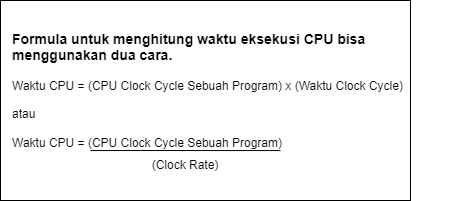
\includegraphics[width=\linewidth]{asset/image1.png}
    \caption{Rumus waktu CPU}
\end{figure}


\hspace*{1cm} Karena waktu eksekusi CPU merupakan hasil dari kedua faktor ini, kita dapat meningkatkan kinerja dengan mengurangi durasi waktu \textit{clock cycle} atau jumlah \textit{clock cycle} yang diperlukan untuk suatu program. Kecepatan \textit{clock} pada dasarnya bergantung pada organisasi CPU tertentu.

\subsubsection{Mengapa \textit{Performance Metrics} Penting}
\hspace*{1cm} Mengukur kinerja menggunakan data yang akurat sangat penting dalam sebuah sistem karena memberikan gambaran nyata tentang performa yang sedang berlangsung. Dengan data yang tepat, manajemen dapat membuat keputusan yang lebih terinformasi, sehingga memperkecil risiko kesalahan dalam strategi. Selain itu, pengukuran kinerja juga membantu mengidentifikasi area yang memerlukan perbaikan, sehingga organisasi dapat berfokus pada peningkatan yang signifikan. Memantau perkembangan dan kemajuan kinerja secara berkala meningkatkan akuntabilitas, baik di tingkat individu maupun tim, sehingga setiap anggota lebih bertanggung jawab atas hasil kerjanya. Pada akhirnya, penggunaan \textit{performance metrics} yang tepat dapat mendorong peningkatan berkelanjutan dengan memberikan dasar yang kuat untuk evaluasi dan inovasi secara sistematis dalam mencapai tujuan jangka panjang.

\subsubsection{Fungsi \textit{Performance Metrics} pada Sistem}
\hspace*{1cm} \textit{Performance metrics} berperan penting dalam berbagai aspek sistem operasi. Berikut adalah beberapa area di mana \textit{performance metrics} digunakan:
\begin{itemize}
    \item \textbf{\textit{Benchmark}} \newline
    \hspace*{1cm} \textit{Benchmark} biasanya menggunakan berbagai \textit{performance metrics} untuk mengukur dan melaporkan hasil kinerjanya. Misalnya, sebuah \textit{benchmark} untuk prosesor mungkin mengukur metrik seperti kecepatan \textit{clock}, jumlah instruksi per detik (\textit{IPS}), atau waktu komputasi untuk tugas tertentu.
    \item \textbf{\textit{Bandwidth}} \newline  
    \hspace*{1cm} Mengukur jumlah data yang dapat ditransmisikan melalui jaringan dalam jangka waktu tertentu. \textit{Bandwidth} yang terbatas membatasi kemampuan sistem untuk menangani banyak permintaan atau mentransfer data dalam jumlah besar, yang pada akhirnya memperlambat waktu muat atau respons. Pada sistem yang sangat bergantung pada transfer data, seperti aplikasi berbasis web atau layanan \textit{cloud}, \textit{bandwidth} adalah faktor penting yang memengaruhi performa keseluruhan.
    \item \textbf{\textit{Error Rate}} \newline  
    \hspace*{1cm} Menghitung persentase permintaan yang gagal diproses atau menghasilkan kesalahan. Metrik ini penting untuk menilai stabilitas dan keandalan sistem. Tingkat kesalahan yang tinggi menunjukkan masalah pada sistem, seperti bug dalam perangkat lunak, kesalahan konfigurasi, atau keterbatasan sumber daya. Tingkat kesalahan yang tinggi dapat mengganggu pengguna dan menurunkan kepercayaan mereka terhadap sistem.
    \item \textbf{Pengaturan Kualitas Layanan (\textit{QoS})} \newline  
    \hspace*{1cm} Dalam lingkungan yang membutuhkan kualitas layanan tertentu, \textit{performance metrics} digunakan untuk memastikan bahwa aplikasi dan layanan memenuhi \textit{SLA} (\textit{Service Level Agreement}). Metrik seperti latensi, \textit{throughput}, dan waktu respons digunakan untuk mengatur dan memantau \textit{QoS}.
    \item \textbf{Optimasi dan Tuning} \newline  
    \hspace*{1cm} \textit{Performance metrics} digunakan untuk mengidentifikasi peluang optimasi dan tuning. Misalnya, dengan
\end{itemize}

\hspace*{1cm} \textit{Performance metrics} berperan penting dalam berbagai aspek pengelolaan dan operasional sistem operasi. Dari monitoring dan manajemen sumber daya hingga optimasi, diagnosis, dan keamanan, metrik ini memberikan wawasan yang diperlukan untuk menjaga sistem tetap berjalan dengan efisien, aman, dan sesuai dengan kebutuhan kinerja yang diharapkan.

\subsection{System Architecture of Computer Systems}
Describes the architecture of modern computer systems, focusing on the interaction between hardware and the operating system.

\subsection{Process Description and Control}
Processes are a central concept in operating systems. This section covers:
\begin{itemize}
    \item Process states and state transitions
    \item Process control block (PCB)
    \item Context switching
\end{itemize}

\subsection{Scheduling Algorithms}
This section covers:
\begin{itemize}
    \item First-Come, First-Served (FCFS)
    \item Shortest Job Next (SJN)
    \item Round Robin (RR)
\end{itemize}
It explains how these algorithms are used to allocate CPU time to processes.

\subsection{Process Creation and Termination}
Details how processes are created and terminated by the operating system, including:
\begin{itemize}
    \item Process spawning
    \item Process termination conditions
\end{itemize}

\subsection{Introduction to Threads}
This section introduces the concept of threads and their relation to processes, covering:
\begin{itemize}
    \item Single-threaded vs. multi-threaded processes
    \item Benefits of multithreading
\end{itemize}

\subsection{File Systems}
File systems provide a way for the operating system to store, retrieve, and manage data. This section explains:
\begin{itemize}
    \item File system structure
    \item File access methods
    \item Directory management
\end{itemize}

\subsection{Input and Output Management}
Input and output management is key for handling the interaction between the system and external devices. This section includes:
\begin{itemize}
    \item Device drivers
    \subsubsection{Teknik Buffering}
    \begin{itemize}
        \item Single Buffering
        \par Merupakan teknik paling sederhana. Ketika proses memberi perintah untuk perangkat
 I/O, sistem operasi menyediakan buffer memori utama sistem untuk operasi. Untuk
 perangkat berorientasi blok. Transfer masukan dibuat ke buffer sistem. Ketika transfer
 selesai,proses memindahkan blok ke ruang pemakai dan segera meminta blok lain.Teknik
 ini disebut reading ahead atau anticipated input.Teknik ini dilakukan dengan harapan
 blok akan segera diperlukan. Untuk banyak tipe komputasi, asumsi ini berlaku. Hanya
 di akhir pemrosesan maka blok yang dibaca tidak diperlukan.
 \newline Keunggulan:
    \begin{itemize}
        \item  Meningkatkan kecepatan karena proses
 dapat memproses data sementara blok
 berikutnya sedang dibaca.
 \item Sistem operasi dapat melakukan swapping
 karena data berada di memori sistem.
    \end{itemize}
    \newline Kekurangan:
    \begin{itemize}
        \item Memperumit sistem operasi karena harus
        mengelola buffer.
        \item Logika swapping terpengaruh, terutama jika
        melibatkan disk I/O.
    \end{itemize}
    \item Double Buffering
    \par Peningkatan dapat dibuat dengan dua buffer sistem.Proses dapat ditransfer ke/dari satu
    buffer sementara sistem operasi mengosongkan (atau mengisi) buffer lain. Teknik ini
    disebut double buffering atau buffer swapping. Double buffering menjamin proses tidak
    menunggu operasi I/O. Peningkatan ini harus dibayar dengan peningkatan kompleksitas.
    \newline Keunggulan & Kelemahan 
    \begin{itemize}
        \item  Meningkatkan efisiensi I/O, namun
        dengan peningkatan kompleksitas
        sistem.
    \end{itemize}
    \item Circular Buffering
    \par  Seharusnya melembutkan aliran data antara perangkat I/O dan proses. Jika kinerja
 proses tertentu menjadi fokus kita, maka kita ingin agar operasi I/O mengikuti proses.
 Double buffering tidak mencukupi jika proses melakukan operasi I/O yang berturutan
 dengan cepat. Masalah sering dapat dihindari denga menggunakan lebih dari dua buffer.
 Ketika lebih dari dua buffer yang digunakan, kumpulan buffer itu sendiri diacu sebagai
 circulat buffer. Tiap buffer individu adalah satu unit di circular buffer.
\newline
\newline Keterbatasan Double Buffering 
\begin{itemize}
\item  Double buffering tidak cukup jika
proses melakukan operasi I/O secara
berurutan dengan cepat.
\end{itemize}
\newline Solusi
\begin{itemize}
\newline  
\item Menggunakan lebih dari dua buffer untuk
mengatasi masalah tersebut.
\item Circular buffer adalah kumpulan buffer
yang berputar, di mana tiap buffer adalah
satu unit di dalamnya.
    
    
\end{itemize}
\end{itemize}
\subsubsection{Programed I/O}
\par  Pada I/O terprogram, data saling dipertukarkan antara CPU dengan modul I/O. CPU
mengeksekusi program yang memberikan operasi I/O kepada CPU secara langsung,
termasuk status perangkat pengindra, pengiriman perintah pembacaan atau penulisan,
dan pemindahan data. Ketika CPU mengeluarkan perintah ke modul I/O, maka CPU
harus menunggu sampai operasi I/O selesai. Apabila CPU lebih cepat dibandingkan
modul I/O, maka hal ini akan membuang-buang waktu CPU. Dengan menggunakan
interupt driven I/O, CPU mengeluarkan perintah I/O, dilanjutkan dengan mengeksekusi
intstruksi-instruksi lainnya, dan diinterupsi oleh modul I/O apabila instruksi-instruksi
tersebut telah selesai dilaksanakan. Dengan menggunakan I/O terprogram dan I/O
interupt, maka CPU bertanggung jawab atas pengeluaran data dan memori utama untuk
keperluan output dan penyimpanan data di dalam memori utama untuk keperluaninput.
Ada dua bentuk lain dari programmed I/O yaitu:
\begin{itemize}
\item  Direct I/O
\par  Sebagai contoh instrument berbasis computer dengan panel saklar dan indicator.Saklar
berfungsi untuk pemilihan mode operasi oleh operatorinstrument. 
Indikator
diimplementasikan menggunakan LED, yang berfungsi sebagai indicator status
instrument.
\newline 
\par Rangkaian tersebut menggunakan prosesor 8-bit dengan ruang alamat I/O terpisah.
Untuk mengisolasi antara bus data dengan saklar diperlukan rangkaian penyangga.
Penyangga ini diimplementasikan dengan octal buffer, yang dapat menampung delapan
saklar. Bagian terpenting lainnya adalah address decoder, yang meng-enable hanya
jika keluaran address decoder hanya dilewatkan pada saat RD* rendah. Selanjutnya,
melihat apa yang terjadi ketika CPU mengeksekusi instruksi “INPUT”. Dianggap alamat
operand berhubungan dengan port input yang ditetapkan.
\newline
\par Pada awal I/O machine cycle keluaran address decoder adalah rendah. Kemudian, RD*
diaktifkan dan SEL1* juga rendah.Selanjutnya keluaran penyangga bus di-enable.
\newline
\par Setiap rangkaian peyangga mengemudikan setiap jalur dari jalur bus data CPU untuk
memberikan nilai tinggi atau rendah. Hal ini tergantung pada posisi saklar yang
bersangkutan.
\newline 
\item  Polled I/O
\par  Pada polled I/O terlebih dahulu di perlukan pemeriksaan status device I/O. Setelah
system diinisialisasi, program I/O yang berhubungan, yaitu I/O driver, membaca
status device I/O. Kemudian menguji bit status untuk menentukan kondisi operasional
device.Apabila device tidak siap, CPU dapat melompat ke tugas (task) yang
lain. Beberapa saat kemudian, setelah beberapa interval waktu, mengulangi proses
sepertidiuraikan di atas. Interval waktu ini tergantung pada kecepatan divais. Sebagai
contoh printer dengan kecepatan 10 cps lamanya adalah 100 ms.
\newline
\par Pada langkah di atas apabila tidak ada task yang dikerjakan, CPU segera mengulang
kembali untuk membaca dan memeriksa status device. Program I/O keluar “wait
loop”.Sekarang program melakukan transfer data atau bisa disebut melayani device.
I/O Interface Controller hubungan device I/O dengan system computer disediakan
melalui rangkaian standar dalam bentuk chip LSI (large scale integration). Rangkaian
ini dikenal dengan I/O interface controller, pheripheral interface adapter, dan
lain-lain. Dengan adanya komponen ini dapat memudahkan menghubungkan device
I/O yang memiliki karakteristik berbeda dengan system bus umum, tanpa atau
meminimumkan penggunaan perangkat keras yang khusus. Antarmuka yang paling
sederhanaadalahregisterpenyanggasatuwordyangbertindaksebagaiportI/O.
\end{itemize}
\end{itemize}

\subsection{Deadlock Introduction and Prevention}
Explores the concept of deadlocks and methods for preventing them:
\begin{itemize}
    \item Deadlock conditions
    \item Deadlock prevention techniques
\end{itemize}

\subsection{User Interface Management}
This section discusses the role of the operating system in managing the user interface. Topics covered include:
\begin{itemize}
    \item Graphical User Interface (GUI)
    \item Command-Line Interface (CLI)
    \item Interaction between the user and the operating system
\end{itemize}

\subsection{Virtualization in Operating Systems}
Virtualization allows multiple operating systems to run concurrently on a single physical machine. This section explores:
\begin{itemize}
    \item Concept of virtualization
    \item Hypervisors and their types
    \item Benefits of virtualization in modern computing
\end{itemize}


\section{Assignments and Practical Work}
\subsection{Assignment 1: Process Scheduling}
\hspace*{1cm} Implementasikan algoritma penjadwalan \textit{Shortest Job First} (SJF) dan \textit{Round Robin} (RR), lalu bandingkan rata-rata waktu tunggu (\textit{average waiting time}) dan rata-rata waktu penyelesaian (\textit{average turnaround time}) dari kedua algoritma tersebut. Manakah yang lebih baik dalam menangani proses? 
\newline
\newline

\begin{center}
    \underline{JAWABAN}
\end{center}

\textit{Short Job First (SJF) algorithms}
\begin{lstlisting}[language=Python]
    def sjf_non_preemptive(Jumlah_proses):
        Jumlah_proses.sort(key=lambda x: x[1])
    
        waktu_tunggu = 0
        total_waktu_tunggu = 0
    
        for pid, burst_time in Jumlah_proses:
            total_waktu_tunggu += waktu_tunggu
            waktu_tunggu += burst_time
    
        n = len(Jumlah_proses)
        avg_waktu_tunggu = total_waktu_tunggu / n
    
        print(total_waktu_tunggu)
        print(f"\nAverage Waiting Time: {avg_waktu_tunggu}")    
    
\end{lstlisting}

\textit{Round Robin (RR) algorithms}
\begin{lstlisting}[language=Python]
    def round_robin(jumlah_proses, quantum):
        n = len(jumlah_proses)
        remaining_time = [bt for _, bt in jumlah_proses]
        waktu_tunggu = [0] * n
        time = 0
    
        while True:
            done = True
            for i in range(n):
                if remaining_time[i] > 0:
                    done = False
                    if remaining_time[i] > quantum:
                        time += quantum
                        remaining_time[i] -= quantum
                    else:
                        time += remaining_time[i]
                        waktu_tunggu[i] = time - jumlah_proses[i][1]
                        remaining_time[i] = 0
            if done:
                break
    
        avg_waktu_tunggu = sum(waktu_tunggu) / n
        print(f"\nAverage Waiting Time: {avg_waktu_tunggu:.2f}")
    
\end{lstlisting}

\begin{figure}[H]
    \centering
    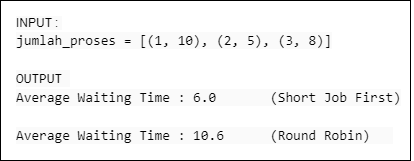
\includegraphics[width=1\linewidth]{asset/41.png}
    \caption{Output}
\end{figure}

\begin{figure}[H]
    \centering
    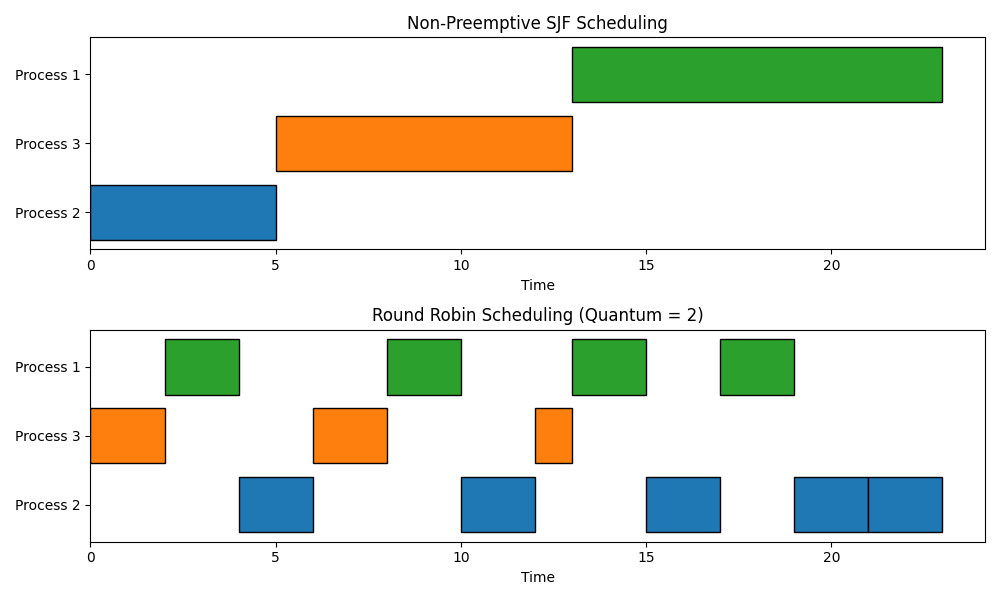
\includegraphics[width=1\linewidth]{asset/411.png}
    \caption{Perbandingan SJF dan RR(quantum = 2)}
\end{figure}

\paragraph{
    \hspace*{1cm} Dari hasil perbandingan rata-rata waktu tunggu pada kedua algoritma, dapat dilihat bahwa rata-rata waktu tunggu SJF lebih kecil dibandingkan dengan \textit{Round Robin}. Salah satu alasannya adalah karena sifat RR yang memberikan setiap proses sejumlah waktu yang sama (\textit{quantum}) dan memaksa semua proses menunggu giliran mereka secara bergantian. 
}

\paragraph{
    \hspace*{1cm} Kita dapat mengurangi kelemahan \textit{Round Robin} dengan memilih \textit{quantum} yang lebih besar. Pada visualisasi di atas terlihat bahwa waktu tunggu RR dapat sama dengan SJF. Namun, tetap saja, SJF sering kali lebih baik dalam kasus dengan banyak proses yang memiliki \textit{burst time} yang bervariasi.
}

\begin{figure}[H]
    \centering
    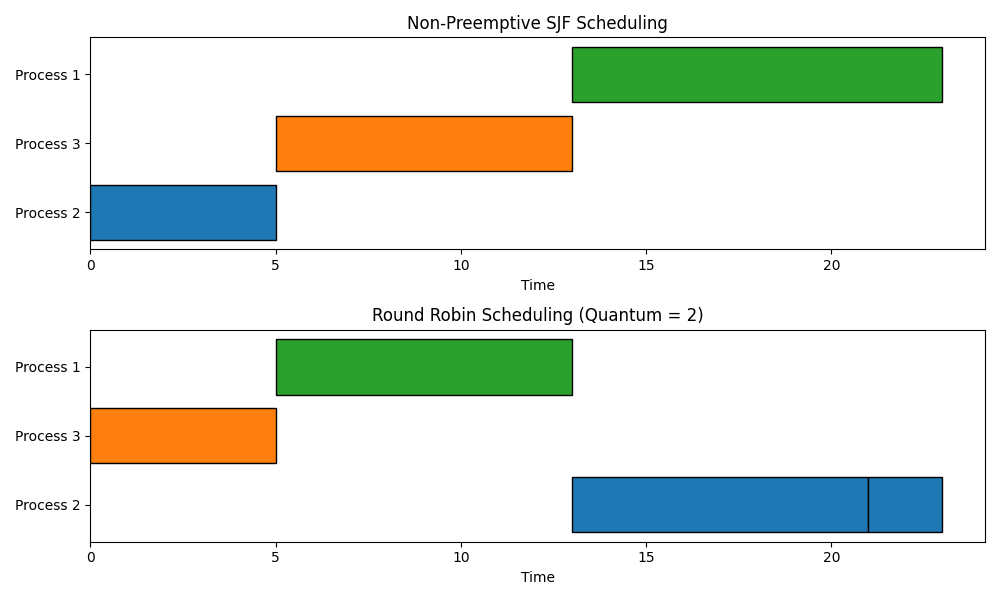
\includegraphics[width=1\linewidth]{asset/412.png}
    \caption{Perbandingan SJF dan RR(quantum = 8)}
\end{figure}


\subsection{Assignment 2: Deadlock Handling}
\hspace*{1cm} Simulasikan bagaimana \textit{algoritma safety} bekerja untuk mendeteksi \textit{deadlock}.
\newline
\newline

\begin{center}
    \underline{JAWABAN}
\end{center}

\begin{lstlisting}[language=Python]

    import numpy as np
    
    def is_safe(Jumlah_proses, avail, max_need, allocation):
        P, R = len(Jumlah_proses), len(avail) 
        need = max_need - allocation 
        finish = [False] * P 
        safe_sequence = []  
        work = avail.copy() 
    
        for _ in range(P):
            for p in range(P):
                if not finish[p] and all(need[p] <= work): 
                    work += allocation[p]
                    finish[p] = True
                    safe_sequence.append(p)
                    break
            else:
                print("Sistem tidak dalam keadaan aman.")
                return False, []
    
        print("Sistem dalam keadaan aman.")
        return True, safe_sequence
    
    
    Jumlah_proses = [0, 1, 2, 3, 4]
    avail = np.array([3, 3, 2]) 
    max_need = np.array([[7, 5, 3],
                         [3, 2, 2],
                         [9, 0, 2],
                         [2, 2, 2],
                         [4, 3, 3]]) 
    allocation = np.array([[0, 1, 0],
                           [2, 0, 0],
                           [3, 0, 2],
                           [2, 1, 1],
                           [0, 0, 2]]) 
    
    is_safe_state, safe_sequence = is_safe(Jumlah_proses, avail, max_need, allocation)
    
    if is_safe_state:
        print("Sistem dalam urutan aman:", safe_sequence)
    else:
        print("Tidak ada urutan aman, sistem dalam keadaan deadlock.")
    
\end{lstlisting}

\begin{figure}[H]
    \centering
    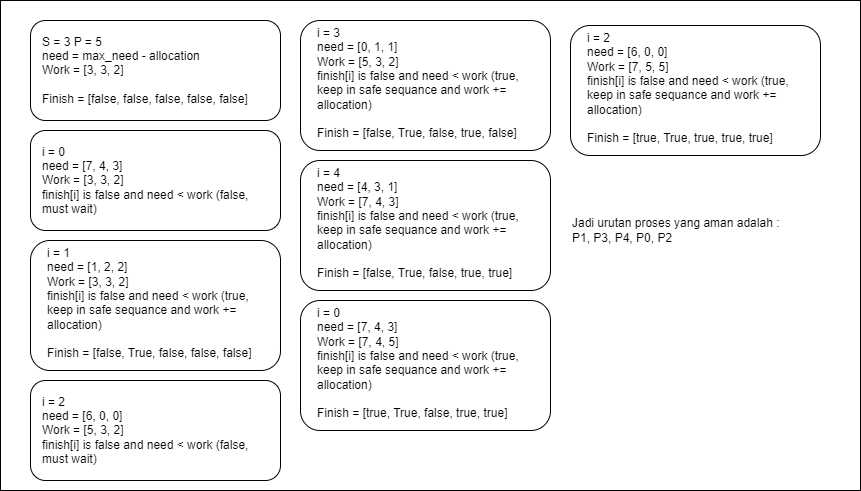
\includegraphics[width=1\linewidth]{asset/421.png}
    \caption{Output dan Penjelasannya}
\end{figure}

\paragraph{
    \hspace*{1cm} Dengan menggunakan metode \textit{Banker's} untuk algoritma \textit{Safety}, kita bisa memastikan bahwa sistem aman jika menjalankan proses-proses tertentu. Di sini, kita memeriksa setiap proses dan memastikan bahwa alokasi sumber daya untuk setiap proses dapat dilakukan dengan aman sehingga tidak akan menyebabkan \textit{deadlock}. Pada output, sistem akan menampilkan status apakah sistem aman atau tidak, dan menampilkan urutan proses yang aman.
}


\subsection{Assignment 3: Multithreading and Amdahl's Law}
\hspace*{1cm} Simulasikan skenario \textit{multithreading} untuk menghitung jumlah kuadrat dari rentang angka yang diberikan dan menjumlahkannya, dan terapkan \textit{Amdahl law} untuk menghitung prediksi kecepatan seiring penambahan \textit{thread} untuk mengetahui penggunaan jumlah \textit{thread} yang optimal.
\newline
\newline

\begin{center}
    \underline{JAWABAN}
\end{center}

\begin{lstlisting}[language=Python]

    import threading
    import time
    
    def compute_squares(start, end, results, index, execution_times):
        start_time = time.time()
        print(f"Thread {index} mulai menghitung dari {start} hingga {end}...")
        result = 0
        for number in range(start, end):
            time.sleep(0.0001) 
            result += number * number
        results[index] = result
        end_time = time.time()
        execution_times[index] = end_time - start_time
        print(f"Thread {index} selesai menghitung dalam {execution_times[index]:.4f} detik.")
    
    total_range = 10000
    num_threads = 4  
    step = total_range // num_threads
    
    
    results = [0] * num_threads
    execution_times = [0] * num_threads
    
    threads = []
    
    start_time = time.time()
    for i in range(num_threads):
        start = i * step
        end = (i + 1) * step if i != num_threads - 1 else total_range
        thread = threading.Thread(target=compute_squares, args=(start, end, results, i, execution_times))
        threads.append(thread)
        thread.start()
    
    for thread in threads:
        thread.join()
    end_time = time.time()
    
    total_execution_time = end_time - start_time
    total_result = sum(results)
    
    def amdahl_law(P, N):
        return 1 / ((1 - P) + (P / N))
    
    
    sequential_fraction = 0.1  
    P = 1 - sequential_fraction
    
    print("Semua thread selesai.")
    print(f"Hasil perhitungan: {total_result}")
    print(f"Waktu eksekusi total: {total_execution_time:.4f} detik")
    
    print("Speedup teoretis menurut Hukum Amdahl:")
    for N in range(1, num_threads + 1):  
        speedup = amdahl_law(P, N)
        print(f"Speedup teoretis dengan {N} thread: {speedup:.2f}x")
    
\end{lstlisting}

\begin{figure}[H]
    \centering
    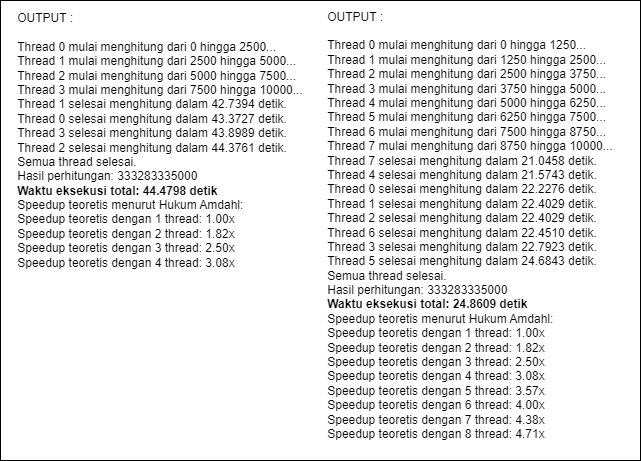
\includegraphics[width=1\linewidth]{asset/31.png}
    \caption{Eksekusi dengan 4 threads (kiri) dan eksekusi dengan 8 threads (kanan)}
\end{figure}

\paragraph{
    \hspace*{1cm} Pada algoritma di atas, \textit{multithreading} berfungsi untuk membagi proses berdasarkan jumlah \textit{thread} yang digunakan, sehingga kita bisa membuat waktu eksekusi menjadi lebih singkat. Dengan menggunakan algoritma \textit{Amdahl's Law}, kita bisa melihat rasio peningkatan kecepatan seiring meningkatnya jumlah \textit{thread} yang digunakan. Dapat dilihat pada perbedaan output di atas, bahwa dengan meningkatkan jumlah \textit{thread} dari 4 ke 8, waktu eksekusi juga meningkat.
}



\subsubsection{Group 9}
\begin{enumerate}
    \item Buatlah program multithreading sederhana dalam Python yang menghitung jumlah bilangan prima dalam rentang tertentu. Kemudian, terapkan Hukum Amdahl untuk menghitung percepatan teoretis berdasarkan proporsi bagian dari program yang dapat diparalelkan.

\textit{JAWABAN : }
\begin{lstlisting}[language=Python, caption={Skenario Multithreading dan Hukum Amdahl}, label={lst:cli_program}, basicstyle=\ttfamily\small, keywordstyle=\color{blue}, commentstyle=\color{gray}]
import threading
import math
import time

def is_prime(n):
    if n <= 1:
        return False
    for i in range(2, int(math.sqrt(n)) + 1):
        if n % i == 0:
            return False
    return True

def count_primes(start, end, results, index):
    count = 0
    for number in range(start, end):
        if is_prime(number):
            count += 1
    results[index] = count

def main():
    start_range = 1
    end_range = 100000
    num_threads = 4
    chunk_size = (end_range - start_range) // num_threads
    threads = []
    results = [0] * num_threads

    for i in range(num_threads):
        start = start_range + i * chunk_size
        end = start_range + (i + 1) * chunk_size if i != num_threads - 1 else end_range
        thread = threading.Thread(target=count_primes, args=(start, end, results, i))
        threads.append(thread)
        thread.start()

    for thread in threads:
        thread.join()

    total_primes = sum(results)
    print(f"Total bilangan prima antara {start_range} dan {end_range} adalah: {total_primes}")

    # Menerapkan Hukum Amdahl
    P = 0.75  # Misalnya 75% dari program dapat diparalelkan
    speedup = 1 / ((1 - P) + (P / num_threads))
    print(f"Percepatan teoretis menggunakan Hukum Amdahl dengan {num_threads} thread: {speedup}")

if __name__ == "__main__":
    main()
\end{lstlisting}
\textit{PENJELASAN: }
\begin{itemize}
    \item \textbf{Import Modul:}
    \begin{itemize}
        \item \texttt{import threading}: Mengimpor modul \texttt{threading} untuk membuat dan mengelola thread.
        \item \texttt{import math}: Mengimpor modul \texttt{math} untuk fungsi matematika, seperti \texttt{sqrt()}.
        \item \texttt{import time}: Modul ini dapat berguna untuk pengukuran waktu, meskipun tidak digunakan dalam kode ini.
    \end{itemize}

    \item \textbf{Fungsi \texttt{is\_prime(n)}:}
    \begin{itemize}
        \item Memeriksa apakah bilangan \texttt{n} adalah bilangan prima dengan cara mengecek faktor dari 2 hingga \texttt{sqrt(n)}. Jika \texttt{n} dapat dibagi oleh salah satu faktor ini, maka \texttt{n} bukan bilangan prima.
    \end{itemize}

    \item \textbf{Fungsi \texttt{count\_primes(start, end, results, index)}:}
    \begin{itemize}
        \item Fungsi ini menghitung jumlah bilangan prima dalam rentang dari \texttt{start} hingga \texttt{end} dan menyimpan hasilnya di \texttt{results} pada indeks \texttt{index}.
    \end{itemize}

    \item \textbf{Fungsi \texttt{main()}:}
    \begin{itemize}
        \item Menentukan rentang pencarian bilangan prima dan jumlah thread yang akan digunakan.
        \item Menghitung \texttt{chunk\_size} untuk membagi rentang pencarian ke dalam bagian yang lebih kecil untuk setiap thread.
        \item Menginisialisasi daftar untuk menyimpan objek thread dan hasil masing-masing thread.
        \item Menggunakan loop untuk membuat dan memulai setiap thread berdasarkan rentang yang ditentukan.
        \item Menunggu semua thread selesai dieksekusi dengan menggunakan \texttt{join()}.
        \item Menghitung total bilangan prima dengan menjumlahkan hasil dari setiap thread dan menampilkannya.
    \end{itemize}

    \item \textbf{Menerapkan Hukum Amdahl:}
    \begin{itemize}
        \item Menerapkan Hukum Amdahl untuk menghitung percepatan teoretis berdasarkan proporsi bagian dari program yang dapat diparalelkan. Misalnya, jika 75\% dari program dapat diparalelkan, maka percepatan teoretis dapat dihitung dengan rumus yang sesuai.
    \end{itemize}
    \end{itemize}
\end{enumerate}

\subsection{Assignment 4: Simple Command-Line Interface (CLI) for User Interface Management}
Students were tasked with creating a simple **CLI** for user interface management. The CLI should support basic commands such as file manipulation (creating, listing, and deleting files), process management, and system status reporting.

\subsubsection{Group 9}
\begin{enumerate}
    \item 

Buatlah sebuah program CLI (Command Line Interface) sederhana menggunakan bahasa pemrograman Python. Program ini harus mendukung perintah-perintah berikut:
\begin{itemize}
    \item Manipulasi file:
    \begin{itemize}
        \item Membuat file baru.
        \item Menampilkan daftar file dalam direktori saat ini.
        \item Menghapus file.
    \end{itemize}
    \item Manajemen proses:
    \begin{itemize}
        \item Menampilkan daftar proses yang sedang berjalan pada sistem.
    \end{itemize}
    \item Pelaporan status sistem
    \begin{itemize}
        \item Menampilkan penggunaan CPU dan memori saat ini.
    \end{itemize}
\end{itemize}
\newline 
Berikut adalah contoh implementasi CLI sederhana menggunakan Python.

\textit{JAWABAN : }
\begin{lstlisting}[language=Python, caption={Program CLI Sederhana}, label={lst:cli_program}, basicstyle=\ttfamily\small, keywordstyle=\color{blue}, commentstyle=\color{gray}]
import os
import psutil  # Untuk manajemen proses dan status sistem

def create_file():
    filename = input("Masukkan nama file yang ingin dibuat: ")
    with open(filename, 'w') as f:
        f.write("")  # Membuat file kosong
    print(f"File '{filename}' berhasil dibuat.")

def list_files():
    files = os.listdir('.')  # Menampilkan daftar file dalam direktori saat ini
    if files:
        print("Daftar file dalam direktori saat ini:")
        for file in files:
            print(file)
    else:
        print("Tidak ada file dalam direktori ini.")

def delete_file():
    filename = input("Masukkan nama file yang ingin dihapus: ")
    if os.path.exists(filename):  # Memeriksa apakah file ada
        os.remove(filename)
        print(f"File '{filename}' berhasil dihapus.")
    else:
        print(f"File '{filename}' tidak ditemukan.")

def list_processes():
    print("Daftar proses yang sedang berjalan:")
    for proc in psutil.process_iter(['pid', 'name']):
        print(f"PID: {proc.info['pid']}, Nama: {proc.info['name']}")  # Menampilkan PID dan nama proses

def system_status():
    cpu_usage = psutil.cpu_percent(interval=1)  # Menghitung penggunaan CPU
    memory_info = psutil.virtual_memory()  # Mendapatkan informasi memori
    print(f"Penggunaan CPU saat ini: {cpu_usage}%")
    print(f"Penggunaan Memori: {memory_info.percent}%")

def main():
    while True:
        print("\nMenu CLI Sederhana:")
        print("1. Membuat file baru")
        print("2. Menampilkan daftar file")
        print("3. Menghapus file")
        print("4. Menampilkan daftar proses yang berjalan")
        print("5. Menampilkan status sistem (CPU & Memori)")
        print("6. Keluar")
        
        choice = input("Pilih perintah (1-6): ")

        if choice == '1':
            create_file()
        elif choice == '2':
            list_files()
        elif choice == '3':
            delete_file()
        elif choice == '4':
            list_processes()
        elif choice == '5':
            system_status()
        elif choice == '6':
            print("Keluar dari program.")
            break
        else:
            print("Pilihan tidak valid, silakan coba lagi.")

if __name__ == "__main__":
    main()
\end{lstlisting}
\textit{PENJELASAN: }
\begin{itemize}
    \item \texttt{import os}: Digunakan untuk manipulasi file dan direktori.
    \item \texttt{import psutil}: Digunakan untuk mendapatkan informasi mengenai proses yang sedang berjalan dan status sistem (penggunaan CPU dan memori).
\end{itemize}

\newline Fungsi \texttt{create\_file()}
\begin{itemize}
    \item Meminta pengguna untuk memasukkan nama file yang ingin dibuat.
    \item Membuat file kosong dengan nama tersebut menggunakan \texttt{with open()}.
\end{itemize}

\newline Fungsi \texttt{list\_files()}
\begin{itemize}
    \item Menggunakan \texttt{os.listdir()} untuk mendapatkan daftar file dalam direktori saat ini.
    \item Menampilkan daftar file kepada pengguna. Jika tidak ada file, mencetak pesan yang sesuai.
\end{itemize}

\newline Fungsi \texttt{delete\_file()}
\begin{itemize}
    \item Meminta pengguna untuk memasukkan nama file yang ingin dihapus.
    \item Memeriksa keberadaan file tersebut dengan \texttt{os.path.exists()}.
    \item Menghapus file jika ada, menggunakan \texttt{os.remove()}.
\end{itemize}

\newline Fungsi \texttt{list\_processes()}
\begin{itemize}
    \item Menggunakan \texttt{psutil.process\_iter()} untuk mendapatkan daftar proses yang sedang berjalan.
    \item Menampilkan PID (Process ID) dan nama setiap proses.
\end{itemize}

\newline Fungsi \texttt{system\_status()}
\begin{itemize}
    \item Menggunakan \texttt{psutil.cpu\_percent()} untuk mendapatkan penggunaan CPU saat ini.
    \item Menggunakan \texttt{psutil.virtual\_memory()} untuk mendapatkan informasi mengenai penggunaan memori.
\end{itemize}

\newline Fungsi \texttt{main()}
\begin{itemize}
    \item Menyediakan menu interaktif bagi pengguna untuk memilih perintah yang diinginkan.
    \item Menggunakan loop \texttt{while True} untuk terus menampilkan menu hingga pengguna memilih untuk keluar dengan opsi 6.
    \item Memproses input pengguna dan memanggil fungsi yang sesuai berdasarkan pilihan yang dibuat.
\end{itemize}
\end{enumerate}

\subsection{Assignment 5: File System Access}
In this assignment, students implemented file system access routines, including:
\begin{itemize}
    \item File creation and deletion
    \item Reading from and writing to files
    \item Navigating directories and managing file permissions
\end{itemize}

\section{Conclusion}
The first half of the course introduced core operating system concepts, including process management, scheduling, multithreading, and file system access. These topics provided a foundation for more advanced topics to be covered in the second half of the course.

\begin{thebibliography}{9}
    \bibitem{gfg2024}
    TestingXperts. (2022, May 10). Performance testing metrics: A detailed guide for businesses. Digital Assurance. Retrieved October 8, 2024, from https://www.testingxperts.com
    \bibitem{gfg2024}
    GeeksforGeeks. (n.d.). Computer organization: Performance of computer. GeeksforGeeks. Retrieved October 1, 2024, from https://www.geeksforgeeks.org/computer-organization-performance-of-computer/
    \bibitem{gfg2024}
    GeeksforGeeks. (2024, August 20). Program for round robin scheduling for the same arrival time. GeeksforGeeks. Retrieved October 8, 2024, from https://www.geeksforgeeks.org/program-for-round-robin-scheduling-for-the-same-arrival-time/
\end{thebibliography}

\end{document}